\documentclass[10pt,conference,compsocconf]{IEEEtran}

%\usepackage{times}
%\usepackage{balance}
\usepackage{url}
\usepackage{graphicx}	% For figure environment
\usepackage{xcolor}
\usepackage{booktabs}

\newcommand\todo[1]{\textcolor{red}{#1}}

\begin{document}
\title{Write-Up Robot Judge}

\author{
  Huber Simon\\
  Department of Computer Science, ETH Zurich, Switzerland
}

\maketitle

\begin{abstract}

\end{abstract}

\section{Introduction}
Topic models are designed to group documents with similar content. A lot of this techniques are unsupervised for multiple reasons: \begin{enumerate}
	\item There is just not enough data that is already labeled. 
	\item The target data set is very small or very specific. 
\end{enumerate} 
But if we interpret hashtags as labeled data for topics then there is already enough data labeled for a very wide range of topics on twitter. With 500 million tweets per day \cite{twitter_stats}. \todo{Figure out how many percent are tagged with a topic.}. The idea then was simple, learn a topic model \todo{explain topic models} through hashtags and apply it to other domains. In this work we were interested in applying it to speeches of politicians. In particular we thought about the following ideas: How does the topics of a speech for a senator change if he is up for reelection ? How are the topics distributed for a democrat or for a republican senator ? Can we use hash tags to predict the party ? And lastly how do the topics compare between speech and twitter for a specific politician and to the general trendy topics ? \\
The paper continuous in the following manor: In section \ref{sec:Plan} we discuss the two models we used to predict the hash tags and why one failed. Then in section \ref{sec:Experiments} we described the planned and executed experiments as well as their result. In section \ref{sec:Discussion} we discuss the results and finally in section \ref{sec:Summary} we summarize and conclude the paper. 

- General Idea
- Hypothesis 
- Paper Structure


\section{Data}
\label{sec:Data}
In this section we present the used datasets, how they were obtained and how they looked. 
\subsection{Twitter Data}
Twitter has the rule that one is not allowed to save tweets along with text. This is because if one wants to make any changes to the tweets e.g. delete them etc. this is no longer globally possible if they are saved somewhere else. So one is only allowed to save them via an unique ID that can be used to retrieve the tweets with the twitter api. A databank full of this tweet ID datasets is found in \cite{twitter_datasets}. We downloaded two datasets.
\subsubsection{Congress Dataset}
The 115th U.S. Congress Tweet Ids dataset contains 2,041,399 tweets. It covers a date distance from 2017-01-27 to 2019-01-02. It therefore covers 1 year before the senate elections and one year after the senate elections which makes it definitely very interesting for us. 
\subsubsection{News Dataset}
The News Outlet Tweet Ids we also downloaded was a fallback dataset which in case the congress dataset was to "fuzzy" could be used to train on more well written, structured and diverse topic distributed dataset. Which was of course just an assumption. 
\subsection{Speeches Data}
The congressional records and therefore the speeches can all be publicly accessed on the congress page \cite{congress_page}. But this side makes it very hard to access specific information. So people developed software packages that parse this side for the information and presents it in an accessible format mostly json. I first tried a package from another student but due to quite a few bugs I had to switch to \cite{congress-downloader} which worked very nicely. I used it to parse all congress information from the years 2017 and 2018. 


\section{Plan}
\label{sec:Plan}
In the first part of this section I will tell shortly about the failure and massive time loss that resulted in trying to adapt LDA to be used with the twitter data and in the second part a short summary of the neural network based method that finally worked for predicting hash tags. 
\subsection{Latent Dirichlet Allocation (LDA)}
\subsubsection{Standard LDA}
LDA was one of the algorithms for topic models that got presented in class. The generative model to generate a word makes it very simple to think about. Given a document sample a topic and for this topic sample a word. And the word is the thing we observe and we can use to learn the corresponding distributions. 
\begin{figure}
	\centering
	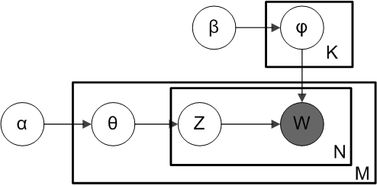
\includegraphics[width=0.7\linewidth]{images/lda_plate}
	\caption{Plate notation for LDA with Dirichlet distributed topic-word distributions.}
	\label{fig:ldaplate}
\end{figure}

\subsubsection{Extended LDA}
So naturally I thought it should be simple to extend LDA so that it can also predict hash tags in the following way. For some document and its document-topic distribution I sample 2 topics and then for the topic-word distribution I sample a word and additionally to the topic-word distribution I just have an topic-hashtag distribution of which I sample a hashtag. And the we can learn the correct distributions since we observe both word and hashtag. 
\begin{figure}
	\centering
	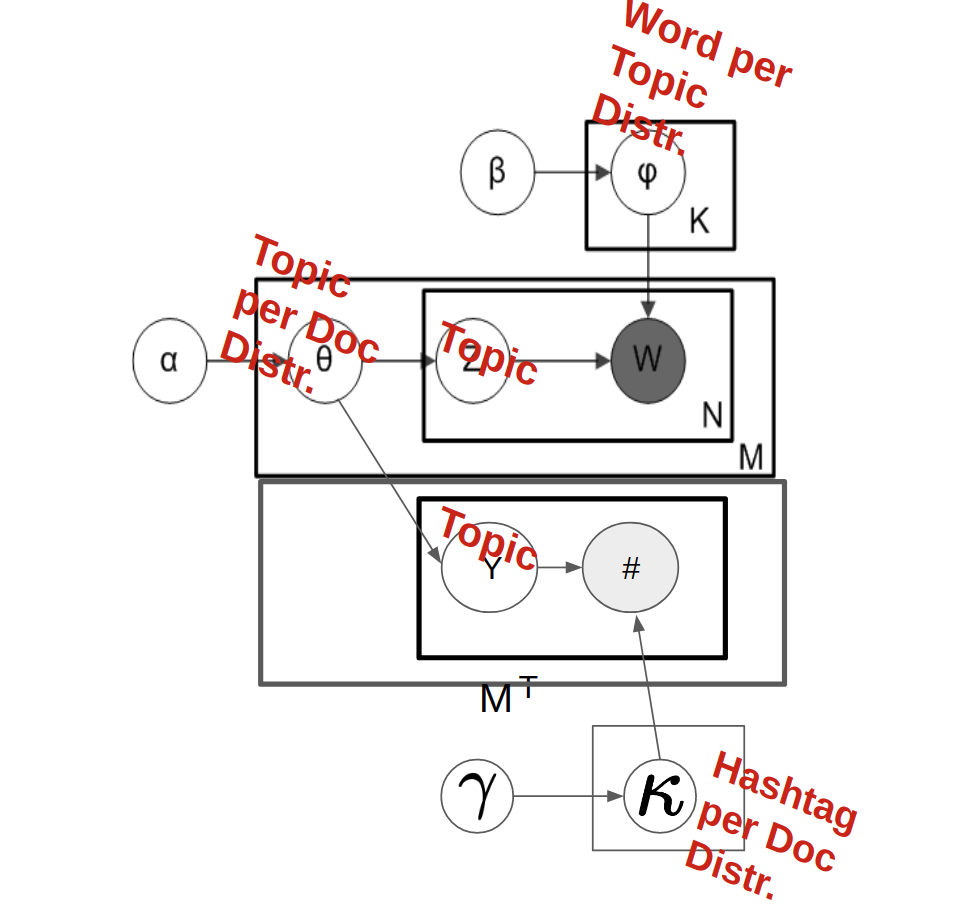
\includegraphics[width=0.7\linewidth]{images/extended_lda}
	\caption{Plate diagram of extended version of LDA with additional distribution for hashtags for a given topic. }
	\label{fig:ldaplate}
\end{figure}

\subsection{Training}
The plan ready I had to find some framework that allowed me to implement and train this generative model. I decided to use pyro \cite{bingham2018pyro} which allows to describe the generative model in a very pytonian way and uses pyTorch \cite{paszke2017automatic} as backend for matrix and optimization calculations which makes it ideal for big datasets. \todo{rename https://github.com/SimiPro/robotjudge/blob/master/Untitled.ipynb and cite as pyro implementation}. The implementation can be seen in \todo{cite my pyro impl. }. But it just didn't work. I tried a multitude of different proposal distributions and even neural networks. It just didn't really converge nicely. I initially thought that the problem was my extension on top of LDA. But it didn't work for LDA aswell. 

\subsection{Tweet2vec - Recurrent Neural Network}
After the extended LDA somewhat failed I tried a multitude of other models. The one that finally worked was a neural network based solution: Tweet2Vec \cite{DhingraZFMC16}. The basic idea behind this model is that they view the character as smallest unit rather then the word as in LDA. This brings quite a few advantages: \todo{How many unique words are in the twitter dataset ? Which makes it difficult to use word based systems. }. Furthermore they assume that a tweet has some latent representation and from this latent representation they predict the hashtag. To get a loss they use cross entropy loss based on predicted hashtag versus given hashtag. The neural network is mainly built out of Bi-directional Gated Recurrent Unit (Bi-GRU) which behave similarly as LSTM's (Long short-term memory) blocks. The size of the input is reasonable constraint on the number of characters a tweet can have - 145. The embedding part of the tweet2vec neural network can be seen in Figure \ref{fig:tweet2vecembedding}. The decoder part is just a dense layer with the number of neurons equal to the number of hashtags. The output of this dense layer is then used as input for the softmax function to get the probability of each hashtag. 
\begin{figure}
	\centering
	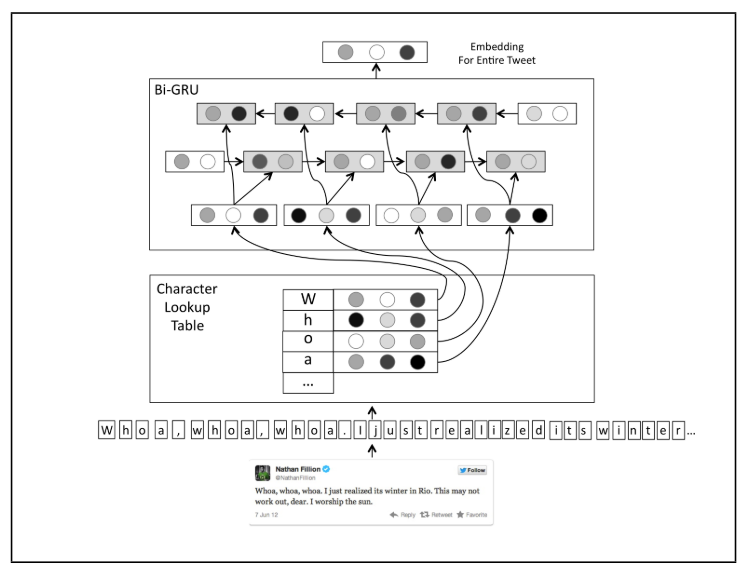
\includegraphics[width=0.7\linewidth]{images/tweet2vec_embedding}
	\caption{Tweet2vec embedding part of the neural network.}
	\label{fig:tweet2vecembedding}
\end{figure}

% Please add the following required packages to your document preamble:
% \usepackage{booktabs}
\begin{table}[]
	\centering
	\begin{tabular}{@{}lll@{}}
		\toprule
		Name       & Party      & Num. Speeches \\ \midrule
		Feinstein  & D   &       2        \\
		Stabenow   & D   &       1        \\
		Klobuchar  & D   &     1          \\
		Menendez   & D   &     1          \\
		Cantwell   & D   &      1         \\
		Warren     & D   &   1            \\
		Gillibrand & D   &        1       \\
		Tester     & D   &     1          \\
		Manchin    & D   &      1         \\
		Murphy     & D   &     5          \\
		Baldwin    & D   &       1        \\
		Hirono     & D   &        1       \\
		Carper     & D   &      1         \\
		Sanders    & I   &      1         \\
		Kaine      & D   &         1      \\
		Brown      & D   &      3         \\
		Heinrich   & D   &       1        \\
		Whitehouse & D   &     1          \\
		Casey      & D   &     1          \\
		Wicker     & R &         0      \\
		Barrasso   & R &    2           \\
		Fischer    & R &         1      \\
		Cruz       & R &      2         \\
		King       & I &     3          \\ \bottomrule
	\end{tabular}
	\caption{List of senators up for reelection in 2018. (D = Democrat, R = Republican, I = Independent)}
	\label{tbl:senators}
\end{table}


\section{Experiments \& Results}
\label{sec:Experiments}
First lets reiterate more concrete about what we want to figure out and then subsequently how we design the experiments to test our hypothesis. 
We start with a simple one: Can we tag speeches of politicians with hashtags learned from twitter ? Then we go on to figure out how tags compare for someone giving a speech before and after campaigning for reelection. 

\subsection{Can we tag speeches of politicians with hashtags learned from twitter ? }
\subsubsection{Data}
As explained in previous sections I used tweet2vec. The politician set consisted of 449334 tweets which we splitted randomly into 90\% training data and 10\% testing data. I counted all the hashtags and removed all that were not in the top 500 used hashtags (from 39671 total).  In Figure \ref{fig:tweet2vectraining} one can see that we got nearly 25\% recall for tag number 1 which is quite good considering how difficult the task is (Randomly predicting one of the top 500 would result in 0.2\% recall). For the speeches I only was interested in the senators up for re-election. It is a set of 24 senators listed in table with their corresponding party and the number of speeches they gave in the years 2017 and 2018. \ref{tbl:senators}. \\
It becomes very obvious that the dataset of speeches is very small. But it does not hinder us to tag the available speeches. To tweet2vec to be able to work on the speeches I had to cut it up into pieces of 145 and additionally I did some preprocessing like stemming, removing stop words and removing line breaks just to get a bit shorter speeches and get more content into those 145 characters.  \todo{add example of speech parts and its tags}

\subsubsection{Results}

 
\subsection{Hashtag analysis}


\subsection{Tweet2vec}


\subsection{Tweet2Vec}
\begin{figure}
	\centering
	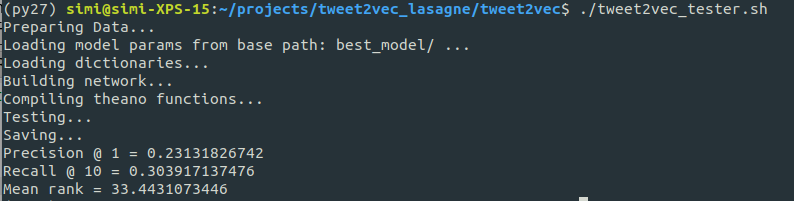
\includegraphics[width=0.7\linewidth]{images/tweet2vec_training}
	\caption{"Proof" of training for tweet2vec.}
	\label{fig:tweet2vectraining}
\end{figure}

\section{Negative Results}


\section{Discussion}
\label{sec:Discussion}

\section{Summary}
\label{sec:Summary}



\bibliographystyle{IEEEtran}
\bibliography{robot_writeup}
\end{document}
